\documentclass[a4paper,10pt]{article}
\usepackage[utf8]{inputenc}
\usepackage{graphicx}
\usepackage{caption}
\usepackage{subcaption}
\usepackage{mathrsfs}
\usepackage{amsmath}

\newcommand{\dd}{\ensuremath{\text{d}}}

\title{Model-free control of underactuated robots with vision-based monitoring}
\author{Thomas Mercier}

\begin{document}

\maketitle

\begin{abstract}

\end{abstract}

\section{Dynamic model}

\begin{figure}
    \centering
    \begin{subfigure}[b]{0.45\textwidth}
        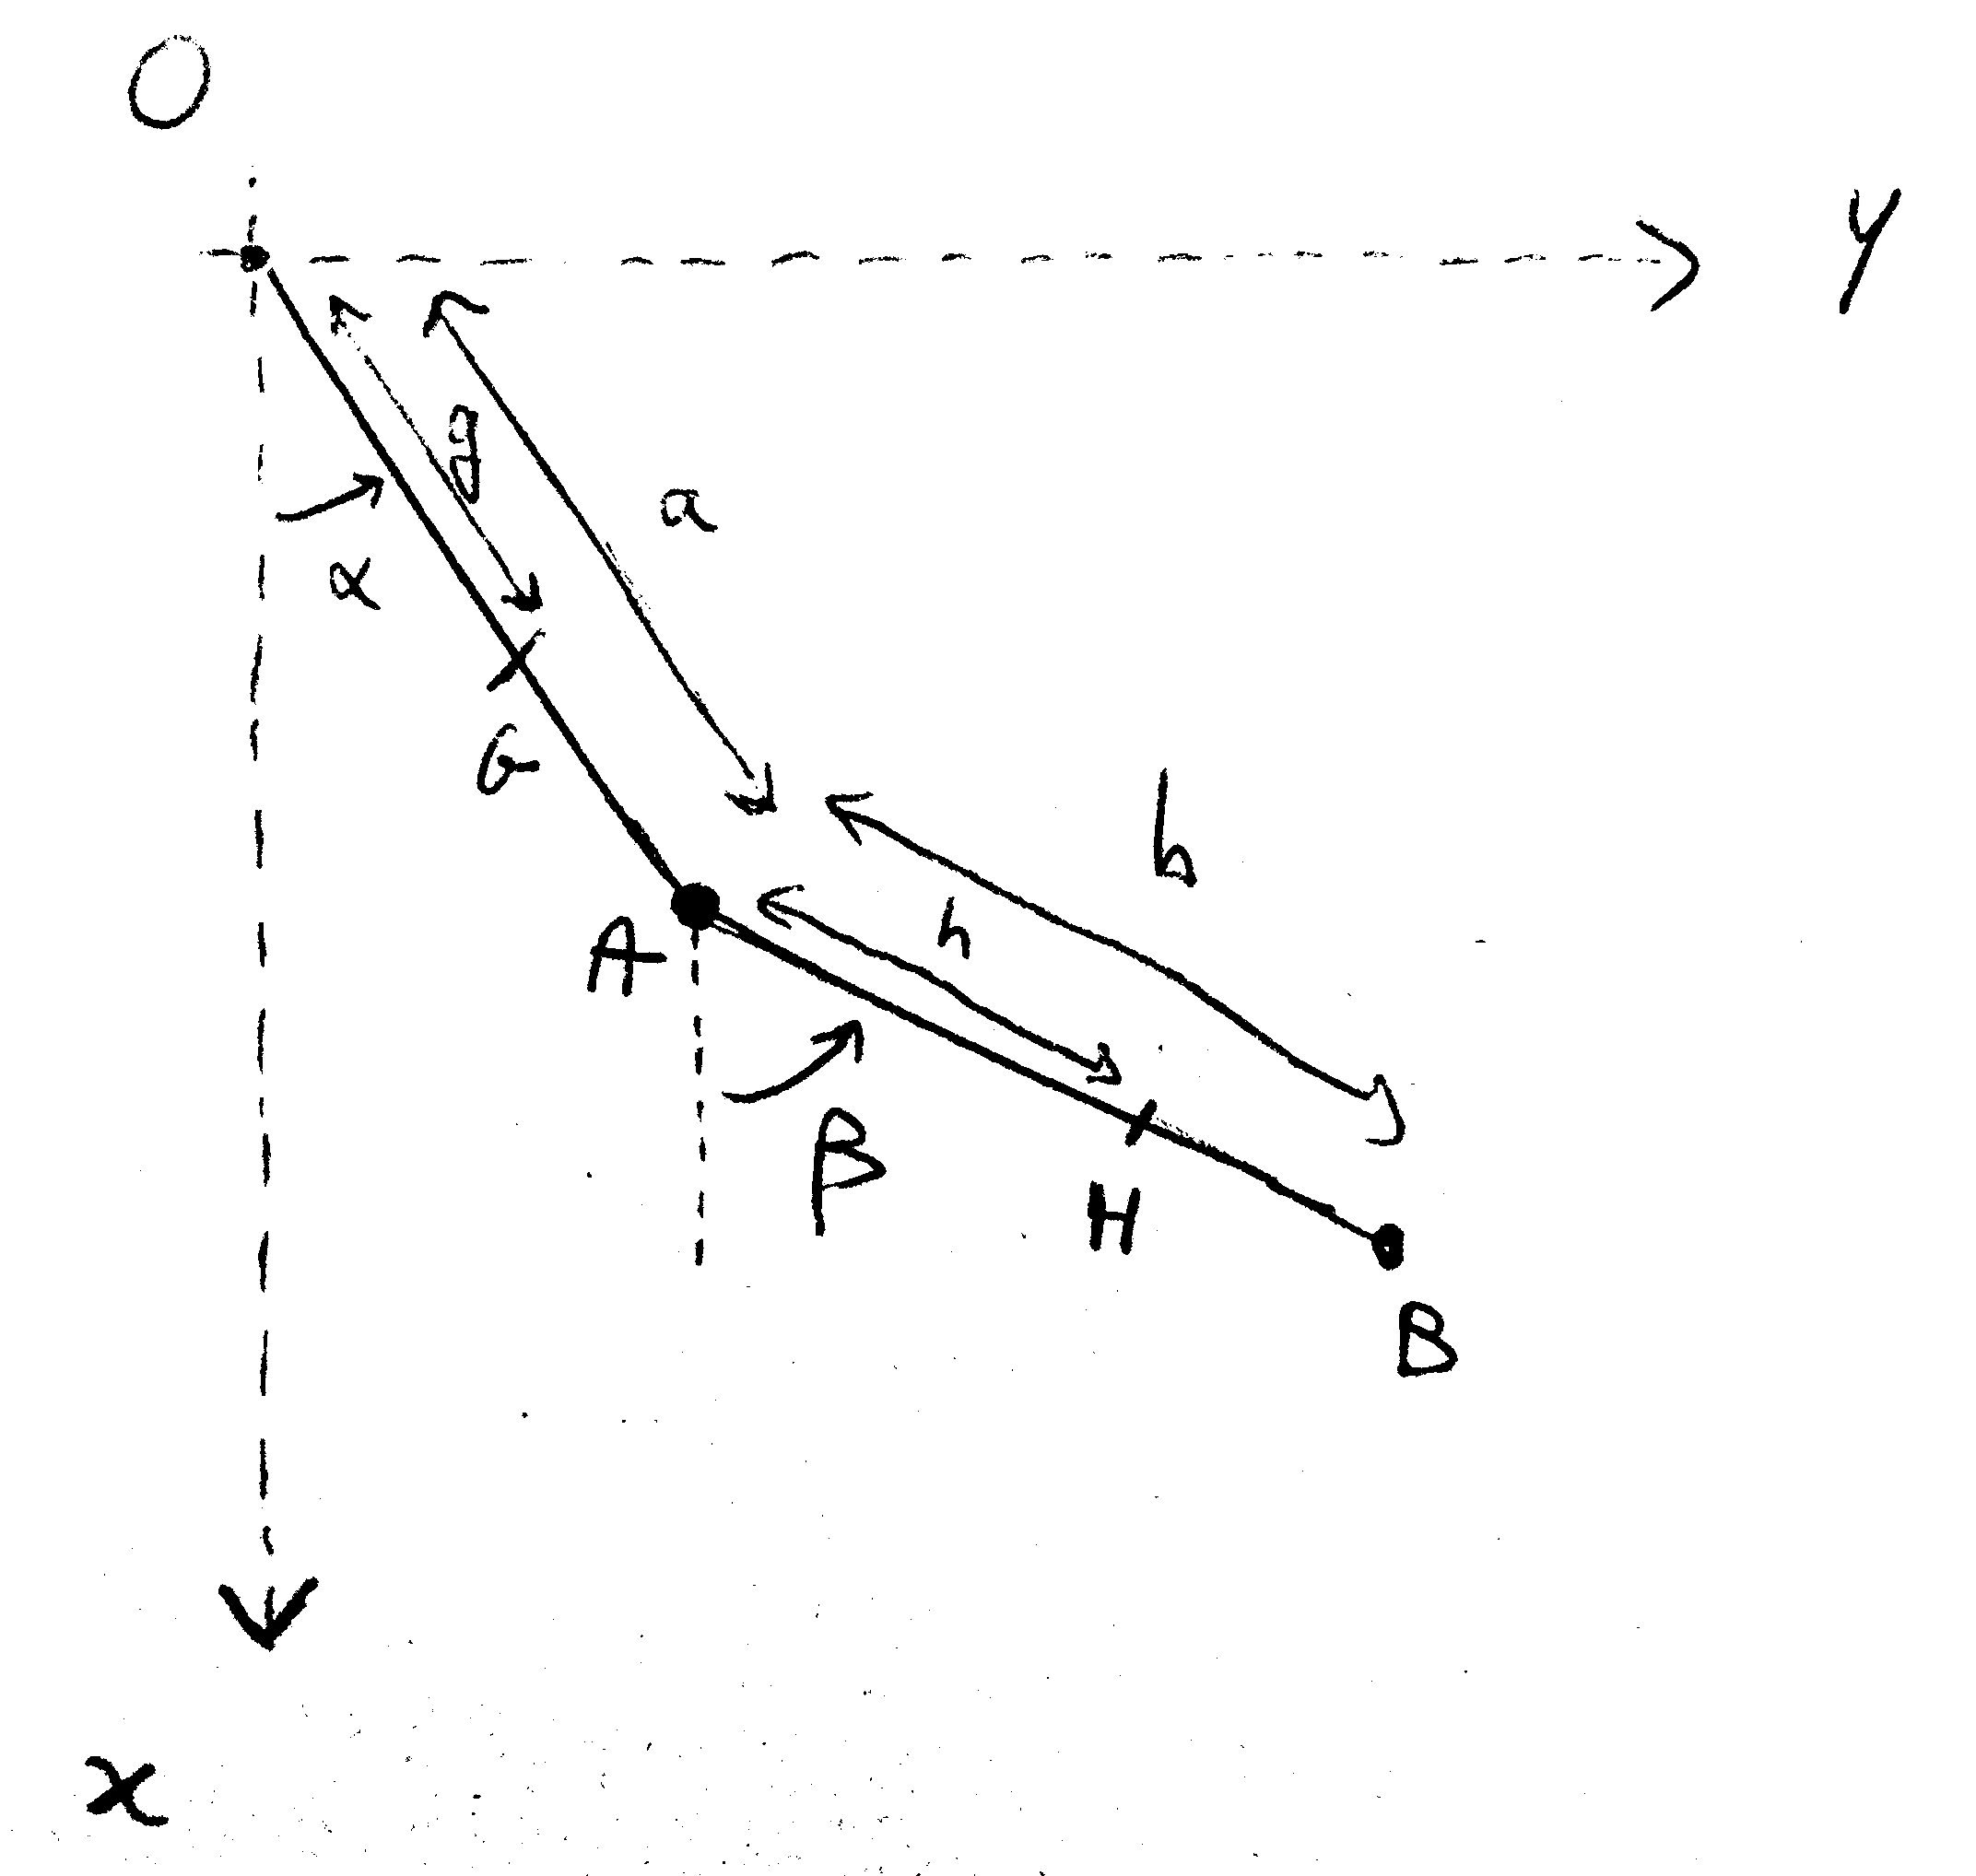
\includegraphics[scale=0.05]{fig/dynamics-double-pendulum.png}
        \caption{Parameterization}
        \label{fig:double-pendulum-param}
    \end{subfigure}
    ~
    \begin{subfigure}[b]{0.45\textwidth}
        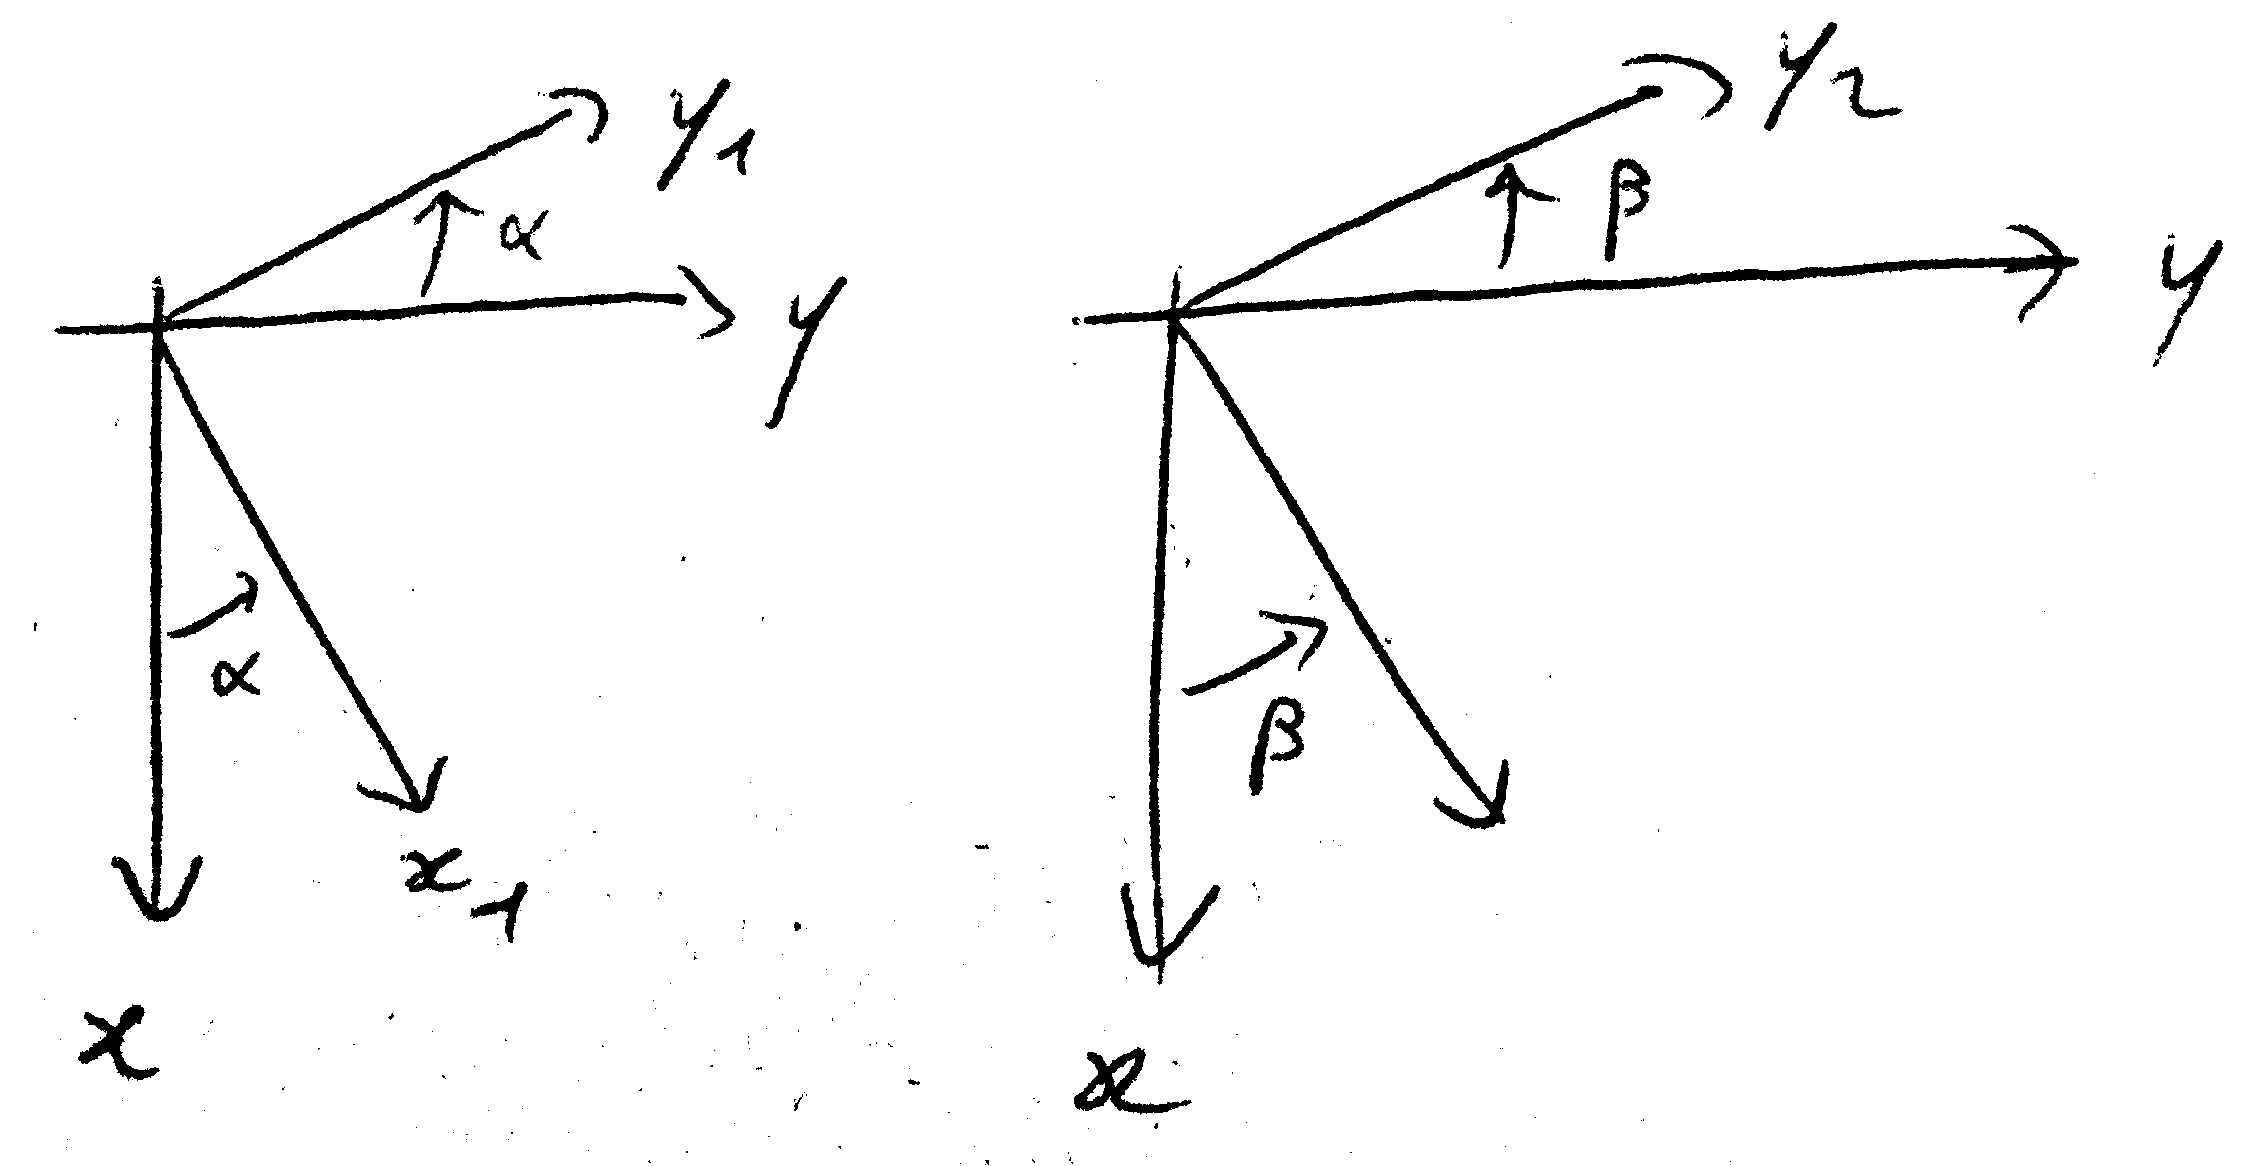
\includegraphics[scale=0.05]{fig/dynamics-angles.png}
        \caption{Local basis}
        \label{fig:double-pendulum-basis}
    \end{subfigure}
    \caption{Double pendulum}\label{fig:double-pendulum}
\end{figure}

\begin{table}
  \begin{tabular}{c|l}
    parameter & description \\
    \hline
    $O$ 		& first hinge \\
    $A$ 		& second hinge \\
    $G$ 		& center of mass of the first mobile \\
    $H$ 		& center of mass of the second mobile \\
    $\alpha$ 		& angle of the first mobile with respect to the reference frame \\
    $\beta$ 		& angle of the first mobile with respect to the reference frame \\
    $m_1$		& mass of the first mobile \\
    $m_2$		& mass of the second mobile \\
    $I_G$		& inertia of the first mobile about its center of mass \\
    $I_H$		& inertia of the second mobile about its center of mass \\
    $a$			& distance $OA$ \\
    $b$			& distance $AB$ \\
    $c$			& distance $OG$ \\
    $d$			& distance $AH$
  \end{tabular}
  \caption{Geometric and inertial parameters \label{tab:parameters}}
\end{table}

The double pendulum is modeled with the parameters described figure~\ref{fig:double-pendulum} and table~\ref{tab:parameters}. The kinetic energy
$$ T = \frac{1}{2} m_1 v_G^2 + \frac{1}{2} I_G \dot{\alpha}^2 + \frac{1}{2} m_1 v_G^2 + \frac{1}{2} I_G \dot{\beta}^2 $$
$$ T = \frac{1}{2} K \dot{\alpha}^2 + \frac{1}{2} L \dot{\beta}^2 + M \dot{\alpha} \dot{\beta} \cos(\alpha-\beta) $$
where $K = m_1 c^2 + m_2 a^2 + I_G$, $L = m_2 b^2 + I_H$ and $M = m_2 a b$. The potential energy
$$ V = -m_1 g x_G - m_2 g x_H = P\cos\alpha + Q\cos\beta $$
where $P = -g(m_1 c + m_2 a)$ and $Q = - m_2 g$. The lagrangian $\mathscr{L}(\alpha, \dot{\alpha}, \beta, \dot{\beta}, t) = T-V$ leads to the equations of motion $\frac{\dd}{\dd t} \frac{\partial \mathscr{L}}{\partial \dot{\alpha}} = \frac{\partial \mathscr{L}}{\partial \alpha}$ (idem for $\beta$) which gives
$$ K \ddot{\alpha} + M \dot{\beta}^2\sin(\alpha-\beta) + M \ddot{\beta}\cos(\alpha-\beta) - P \sin(\alpha) = 0 $$
$$ L \ddot{\beta} - M \dot{\alpha}^2\sin(\alpha-\beta) + M \ddot{\alpha}\cos(\alpha-\beta) - Q \sin(\beta) = 0 $$
and can be rewritten
$$ \ddot{\alpha} = \frac{PL\sin\alpha-MQ\sin\beta\cos(\alpha-\beta)-ML\dot{\beta}^2\sin(\alpha-\beta)-M^2\dot{\alpha}^2\sin(\alpha-\beta)\cos(\alpha-\beta)}{LK-M^2\cos^2(\alpha-\beta)} $$
$$ \ddot{\beta} = \frac{KQ\sin\beta-MP\sin\alpha\cos(\alpha-\beta)+MK\dot{\alpha}^2\sin(\alpha-\beta)+M^2\dot{\beta}^2\sin(\alpha-\beta)\cos(\alpha-\beta)}{LK-M^2\cos(\alpha-\beta)} $$
\end{document}
